\section{Вращение твёрдого тела вокруг неподвижной оси}

\subsection{Определение. Основные понятия}

Рассмотрим движение твёрдого тела, при котором две точки его остаются
неподвижными; такое движение представляет собой вращение тела вокруг проходящей
через неподвижные точки прямой, называемой \textit{осью вращения}.

\begin{figure}[H]
  \centering
  \resizebox{\linewidth}{!}{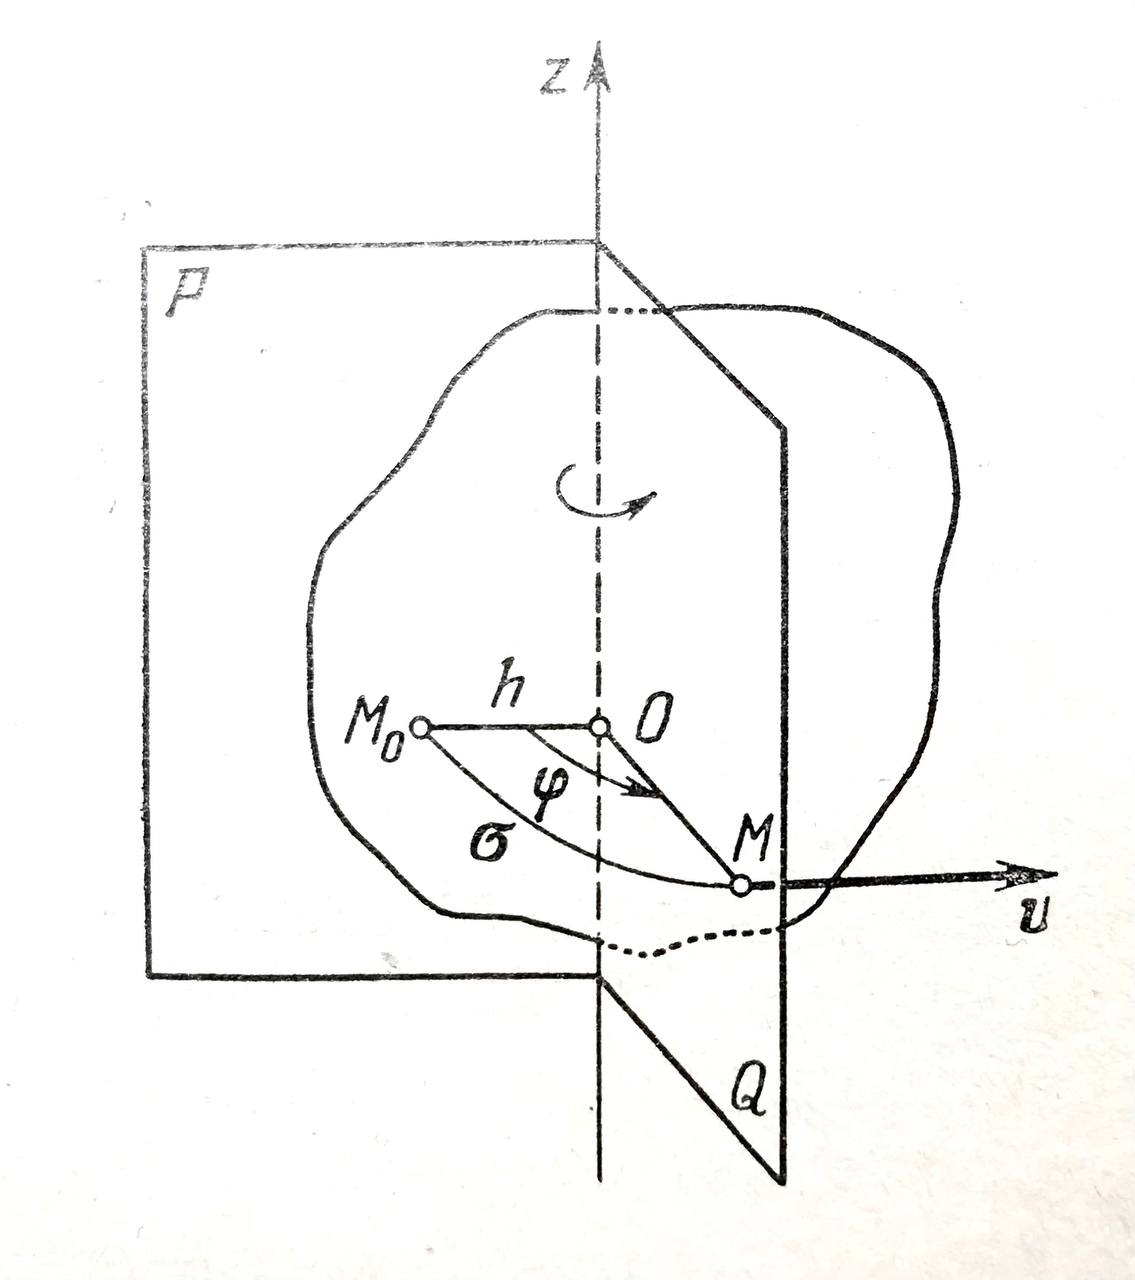
\includegraphics{src/mechanics/pictures/13_1.jpg}}

  \caption{}
  \label{fig:dihedral_angle}
\end{figure}

Пусть ось вращения тела совпадает с осью $Oz$. Чтобы определить положение тела,
проведём через ось $Oz$ две полуплоскости: подвижную $Q$, твёрдо связанную с
вращающимся телом, и неподвижную $P$. Заданием двугранного угла $\varphi$
между этими полуплоскостями положение твёрдого тела вполне определяется.

Движение твёрдого тела, имеющего неподвижную ось вращения, определяется заданием
угла $\varphi$ в функции времени:
\begin{equation}
  \varphi = f(t).
\end{equation}
Это уравнение называется \textit{уравнением вращения} тела.

Величина, учитывающая быстроту изменения угла поворота со временем, называется
\textit{угловой скоростью тела}.

Условимся обозначать абсолютное значение некоторой величины как $a$, а её
алгебраическое значение как $\tilde{a}$. Конечно, $\abs{\tilde{a}} = a$. В
случае угловой скорости будем использовать соответственно обозначения $\omega$
и $\tilde{\omega}$.

За меру быстроты изменения угла поворота с течением времени примем отношение
приращения угла $\Delta \varphi$ к промежутку времени $\Delta t$, в течение
которого это приращение произошло. Такое отношение назовём \textit{средней
угловой скоростью} за промежуток времени $\Delta t$ и обозначим
\begin{equation*}
  \tilde{\omega}_{\text{ср}} = \deltader{\varphi}{t}.
\end{equation*}
Желая перейти от средней угловой скорости за некоторый промежуток времени к
\textit{истинной угловой скорости в данный момент}, будем стремить интервал
времени $\Delta t$ к нулю. По определению производной угловая скорость
$\tilde{\omega}$ в данный момент будет равна
\begin{equation}
  \label{eq:angular_velocity}
  \tilde{\omega} = \lim_{\Delta t \to 0} \tilde{\omega}_{\text{ср}} =
    \lim_{\Delta t \to 0} \deltader{\varphi}{t} = \dt[\varphi] = \dot{\varphi}.
\end{equation}

Аналогично вводится понятие \textit{среднего углового ускорения} за промежуток
времени $\Delta t$:
\begin{equation*}
  \tilde{\varepsilon}_{\text{ср}} = \deltader{\tilde{\omega}}{t}
\end{equation*}
и \textit{углового ускорения в данный момент}:
\begin{equation}
  \label{eq:angular_acceleration}
  \tilde{\varepsilon} = \lim_{\Delta t \to 0} \tilde{\varepsilon}_{\text{ср}} =
    \lim_{\Delta t \to 0} \deltader{\tilde{\omega}}{t} = \dt[\tilde{\omega}] =
    \dot{\tilde{\omega}}.
\end{equation}

Из формулы \ref{eq:angular_velocity} будет также следовать
\begin{equation*}
  \tilde{\varepsilon} = \ddt[\varphi] = \ddot{\varphi}.
\end{equation*}

% TODO: скалярные формулы скорости и ускорения -//-

\subsection{Векторные формулы скорости и ускорения точек твёрдого тела,
вращающегося вокруг неподвижной оси}

Введём в рассмотрение \textit{вектор угловой скорости}, который будем обозначать
через $\vec{\omega}$.

Величиной вектора угловой скорости $\vec{\omega}$ является
\begin{equation*}
  \omega = \abs{\dt[\varphi]} = \dot{\varphi}.
\end{equation*}

Условимся направлять вектор угловой скорости $\vec{\omega}$ по оси вращения так,
чтобы наблюдатель, смотрящий с конца вектора $\vec{\omega}$, видел вращение тела
в положительном направлении, то есть против часовой стрелки при правой системе
координат.

Откладывая вектор $\vec{\omega}$ по оси вращения, можно определить вектор
линейной скорости $\vec{v}$ любой точки $M$ как векторное произведение вектора
угловой скорости на вектор-радиус этой точки относительно любой точки оси
вращения (\textit{формула Эйлера}):
\begin{equation}
  \label{eq:euler_formula}
  \vec{v} = \crossprod{\vec{\omega}}{\vec{r}}.
\end{equation}

\begin{figure}[H]
  \centering
  \resizebox{\linewidth}{!}{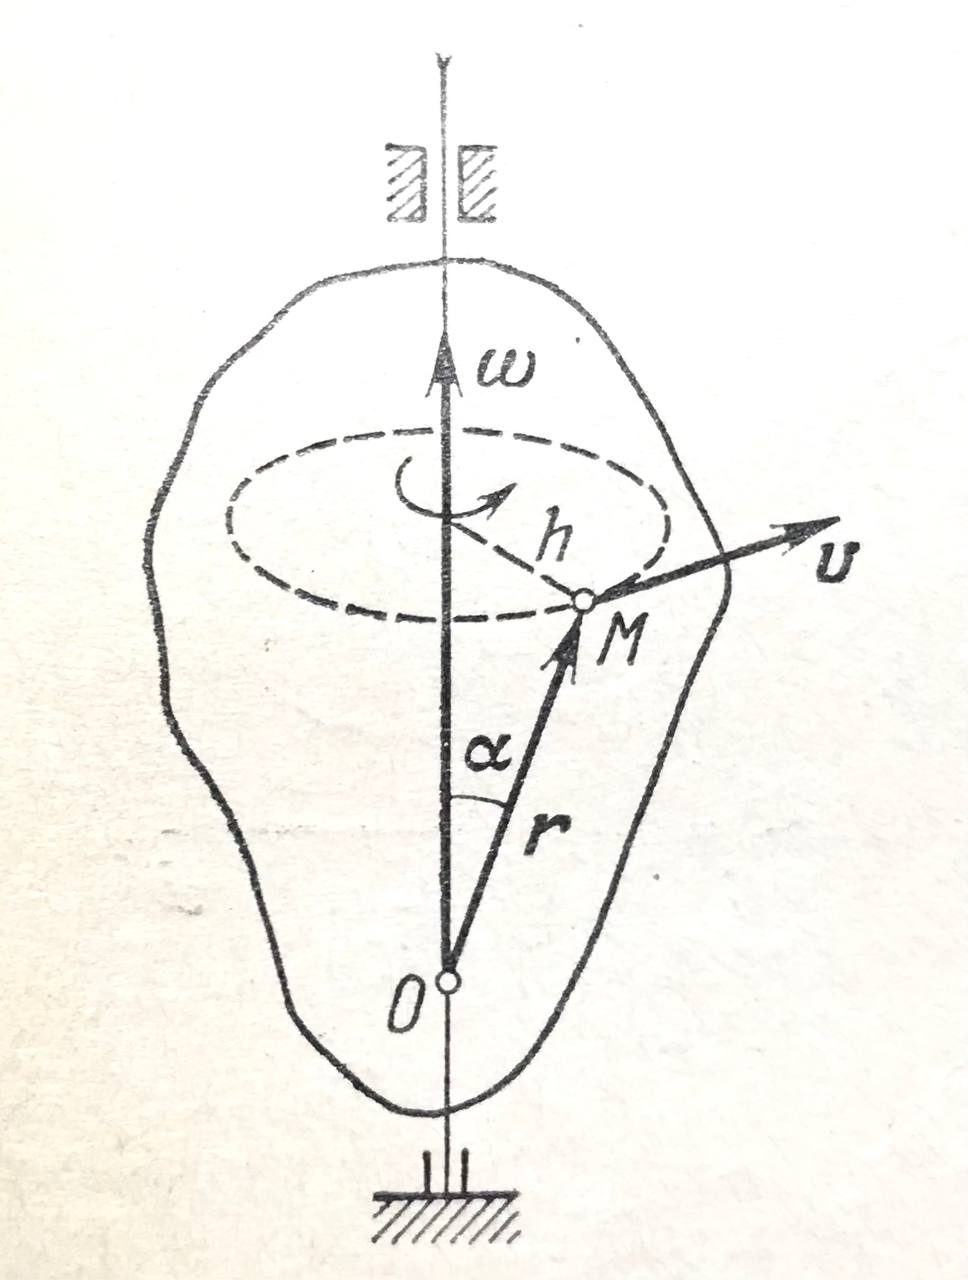
\includegraphics{src/mechanics/pictures/13_2.jpg}}

  \caption{}
  \label{fig:dihedral_angle}
\end{figure}

В самом деле, величина векторного произведения \ref{eq:euler_formula} равна
\begin{equation*}
  v = \omega r \sin \alpha = \omega h,
\end{equation*}
то есть величине скорости; пусть, далее, принята правая система осей, тогда при
показанном стрелкой направлении вращения вектор угловой скорости должен быть
отложен по оси вращения вверх. Векторное произведение
$\vec{\omega} \times \vec{r}$ перпендикулярно к $\vec{\omega}$ и $\vec{r}$ и
направлено так, чтобы, смотря с его конца, видеть поворот от $\vec{\omega}$ к
$\vec{r}$ на наименьший угол против часовой стрелки; но это и будет направление
скорости $\vec{v}$.

Выведем теперь векторную формулу ускорения. Для этого возьмём векторную
производную по времени от обеих частей равенства \ref{eq:euler_formula}; будем
иметь
\begin{equation}
  \label{eq:acceleration_rotation_verbose}
  \vec{w} = \dt[\vec{v}] = \dt (\crossprod{\vec{\omega}}{\vec{r}}) =
    \crossprod{\dt[\vec{\omega}]}{\vec{r}} +
    \crossprod{\vec{\omega}}{\dt[\vec{r}]}.
\end{equation}

Производную по времени от вектора угловой скорости $\vec{\omega}$ назовём
\textit{вектором углового ускорения}. Называя вектор углового ускорения
$\vec{\varepsilon}$ и замечая, что по определению скорости $\dot{\vec{r}} =
\vec{v}$, приведём \ref{eq:acceleration_rotation_verbose} к виду
\begin{equation}
  \label{eq:rotation:acceleration}
  \vec{w} = \crossprod{\vec{\varepsilon}}{\vec{r}} +
    \crossprod{\vec{\omega}}{\vec{v}}.
\end{equation}

Первое слагаемое, $\crossprod{\vec{\varepsilon}}{\vec{r}}$, представляет собой
\textit{вращательную} составляющую ускорения. Действительно, оно равно по
величине
\begin{equation*}
  w^{\text{(в)}} = \varepsilon r \sin(\widehat{\vec{\varepsilon}, \vec{r}})
    = \varepsilon h,
\end{equation*}
а по направлению совпадает со скоростью $\vec{v} =
\crossprod{\vec{\omega}}{\vec{r}}$, если векторы $\vec{\omega}$ и
$\vec{\varepsilon}$ сонаправлены, и противоположно скорости, если $\vec{\omega}$
и $\vec{\varepsilon}$ разнонаправлены.

Второе слагаемое в формуле \ref{eq:rotation:acceleration} представляет собой
\textit{осестремительное} ускорение. Его величина равна
\begin{equation*}
  w^{\text{(ос)}} = \omega v \sin(\widehat{\vec{\omega}, \vec{v}})
    = \omega^2 h,
\end{equation*}
так как векторы $\omega$ и $v$ взаимно перпендикулярны, а $v = \omega h$.

Направление векторного произведения $\crossprod{\vec{\omega}}{\vec{v}}$
перпендикулярно к оси вращения (вектору $\vec{\omega}$) и скорости $\vec{v}$, то
есть идёт по радиусу круга, описываемого точкой, к его центру. Итак,
действительно,
\begin{equation}
  \vec{w}^{\text{(в)}} = \crossprod{\vec{\varepsilon}}{\vec{r}}, \quad
    \vec{w}^{\text{(ос)}} = \crossprod{\vec{\omega}}{\vec{v}}.
\end{equation}

\subsection{Список литературы}
\begin{enumerate}
  \item \cite{lourie}
\end{enumerate}

